\documentclass[a4paper]{scrbook}
\usepackage[utf8]{inputenc} 
\usepackage[upright]{fourier} 
\usepackage[usenames,dvipsnames,svgnames]{xcolor}
\usepackage{tkz-euclide,fullpage}
\usetkzobj{all}
%\usepackage[frenchb]{babel}
\definecolor{fondpaille}{cmyk}{0,0,0.1,0}
\tkzSetUpColors[background=fondpaille,text=Maroon]  

\begin{document} 

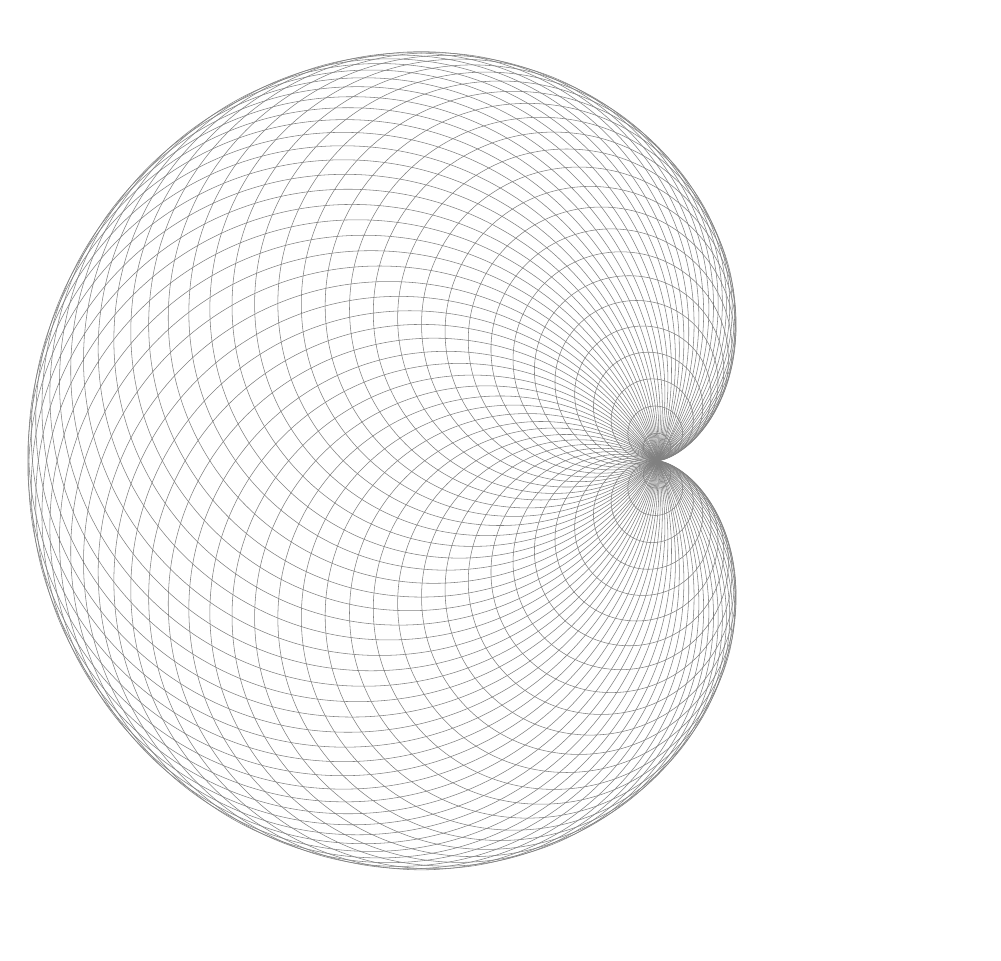
\begin{tikzpicture}
  \tkzInit[xmin=-6,ymin=-6,
           xmax= 6,ymax= 5.5]  
  \tkzClip 
  \tkzDefPoint(0,0){O} 
  \tkzDefPoint(2,0){A}
  \foreach \ang in {5,10,...,360}{%
     \tkzDefPoint(\ang:2){M}
     \tkzDrawCircle[](M,A) 
   }  
\end{tikzpicture} 
\end{document}
